\documentclass[12pt]{article}

\usepackage{graphicx}

\begin{document}
\section{Introductie}
Volgend systeem beschrijft een motor met aan/uit-regeling. Dit systeem bestaat uit een lineair en niet-lineair deel. De regelkring wordt weergegeven in figuur \ref{regellus}.
\begin{figure}[!h]
	\centering
	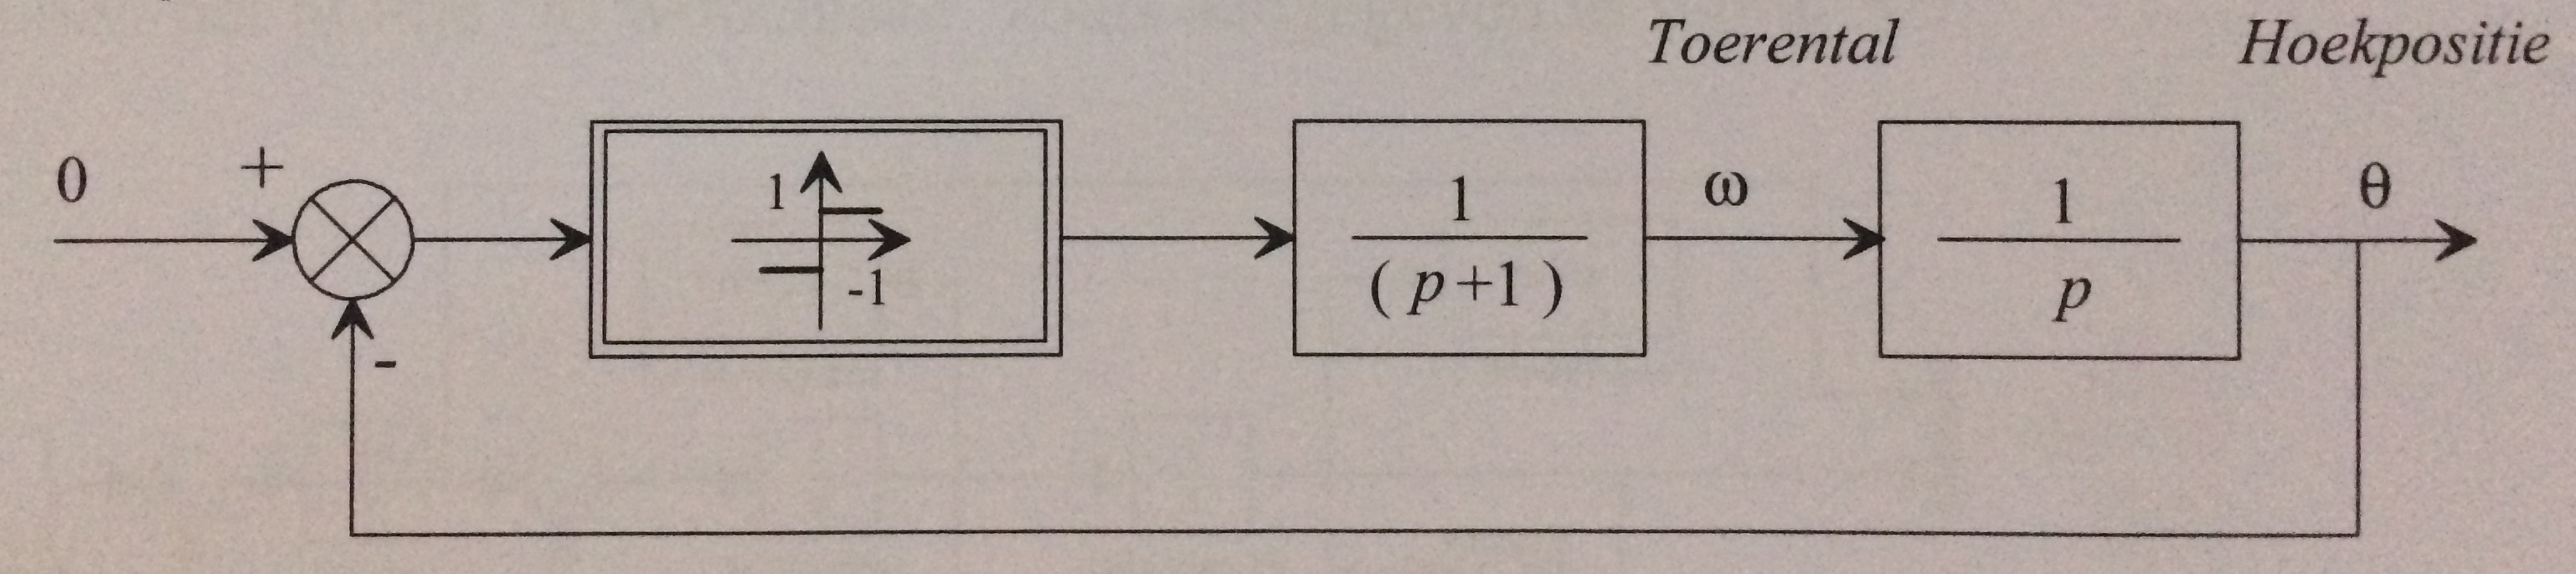
\includegraphics[width=\textwidth, keepaspectratio]{regellus.png}
	\caption{Regellus voor Aan/uit positieregeling}
	\label{regellus}	
\end{figure}

\noindent
Het niet-lineaire deel bestaat uit het aan/uit-element. Deze schakelt tussen de waarden +1 en -1 om de motor respectievelijk positief en negatief te laten draaien. De motor zelf is een eerste orde systeem met transfertfunctie $TF_{motor} = \frac{1}{p+1}$. Hieruit volgt dat $K=1$ en $\tau=1$. Gezien de hoekpositie graag gekend is wordt er tenslotte een zuivere integrator toegevoegd. Immers geldt dat $\theta = \int_{\Delta t} \omega \ \mathrm{d}t$. \\ \\
\section{Simulatie}
Om deze schakeling te simuleren in SIMULINK werd gebruik gemaakt van het schema uit figuur \ref{simulinkschema}. Deze omzetting maakt het mogelijk om de beginwaarden van $\omega$ en $\theta$ te kiezen. Als beginwaarden werden gekozen:
\[ 
\left \{
  \begin{tabular}{c}
  $\omega_0 = 2$ rad/s \\
  $\theta_0 = 1.5$ rad
  \end{tabular}
\right. 
\]
\begin{figure}[]
	\centering
	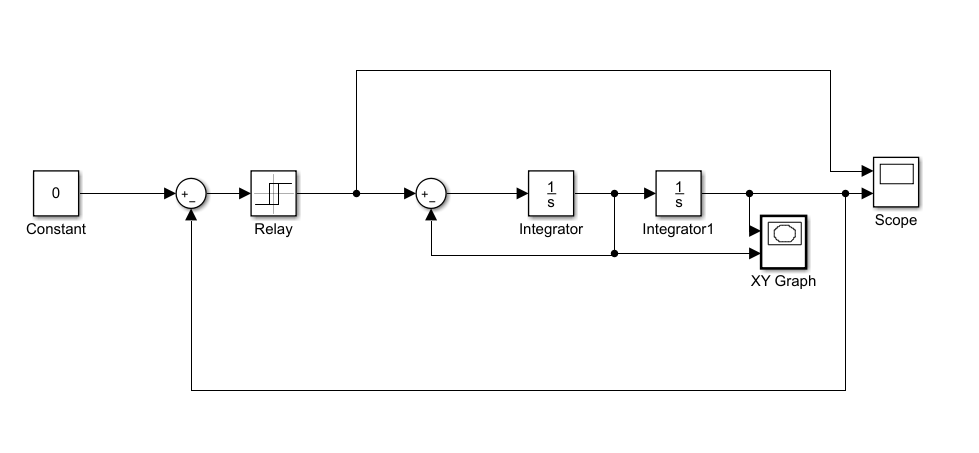
\includegraphics[width=\textwidth, keepaspectratio]{simulinkschema.png}
	\caption{Gesimuleerd schema in SIMULINK}
	\label{simulinkschema}
\end{figure}
Na een simulatie van 10 seconden levert dit de output uit figuur \ref{output1}.
\begin{figure}[]
	\centering
	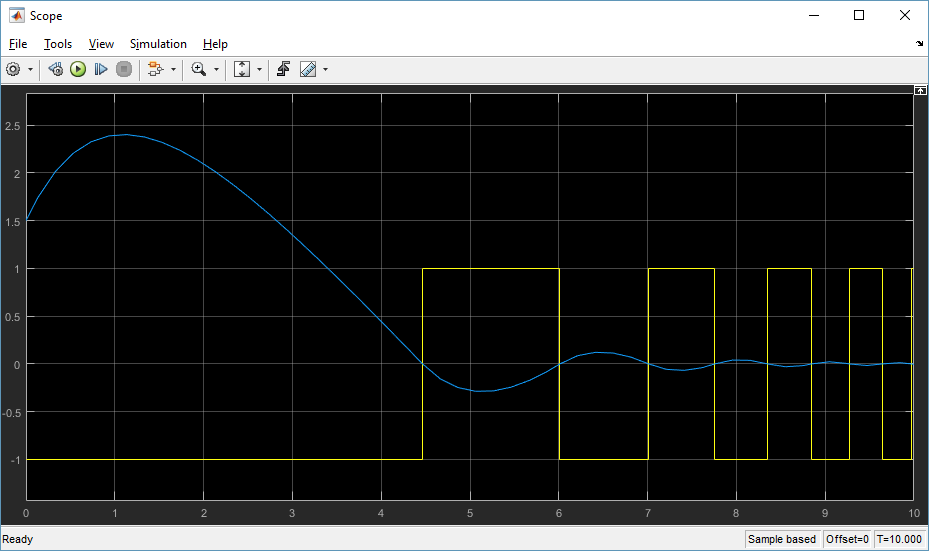
\includegraphics[width=\textwidth, keepaspectratio]{output1.png}
	\caption{Tijdrespons (10 seconden) voor $\omega_0 = 2$ rad/s en $\theta_0 = 1.5$ rad (zonder hysteresis)}
	\label{output1}
\end{figure}
\newpage
\noindent De fasetrajecten worden bepaald door $\omega$ uit te zetten als een functie van $\theta$. Deze waarden zijn rechtstreeks toegankelijk in het schema en worden geplot in een XY-grafiek. Dit levert het resultaat uit figuur \ref{xynohys}. Indien men het fasetraject wil bekomen met hysteresis dient het relais pas aan/uit te schakelen bij een bepaalde waarde. Voor figuur \ref{xyhys} werd een uit/aan-schakelwaarde van $[-0.5;0.5]$ gekozen. \\ \\
Het valt op dat de figuur met hysteresis blijkt te convergeren naar de waarde 0. Dit komt overeen met de gesimuleerde tijdrespons uit figuur \ref{output1}. Hierin blijkt immers ook dat na een langere tijd de outputwaarde convergeert naar 0. Ook blijkt dat het schakelelement (gele lijn) frequenter zal aan/uit schakelen. Dit is ook logisch gezien de outputwaarde constant sneller door 0 zal gaan en de schakelaar dus vaker probeert het systeem te corrigeren. \\ \\
Voor de tijdrespons van het systeem inclusief hysteresis te simuleren werd gebruik gemaakt van volgende waarden:
\[ 
\left \{
  \begin{tabular}{c}
  $\omega_0 = 0.75$ rad/s \\
  $\theta_0 = 1$ rad \\•
  hysteresis = $\pm 0.4$
  \end{tabular}
\right. 
\]
Het fasetraject wordt afgebeeld in figuur \ref{xytwo}. Deze figuur komt overeen met de eerder geziene figuur voor hysteresis. Twee belangrijke verschillen zijn de volgende:
\begin{itemize}
	\item Het beginpunt ligt anders. Deze is afhankelijk van de gekozen beginwaarden. In dit geval ligt het beginpunt op $[1;0.75]$. 
	\item De breedte van de hysteresislus is verkleind. Dit valt te verklaren uit het kleiner gekozen hysteresinterval.
\end{itemize}
De tijdrespons wordt afgebeeld in figuur \ref{output2}. Hierin valt duidelijk de oscillatie te merken. Dit is te danken aan de ingesteld hysteresis. Bij $\theta = \pm 0.4$ zal het schakelelement omschakelen. Dit zorgt ervoor dat de motor zal omkeren. Hoewel deze output een grotere fout vertoont, is deze manier van regelen meer gewenst. In de eerdere figuur viel immers op hoe het schakelelement steeds frequenter begon te schakelen. Dit zorgt ervoor dat dit element sneller tot aan zijn maximale schakelfrequentie zal geraken, met stuk gaan tot gevolg. 
\newpage
\begin{figure}[!h]
	\centering
	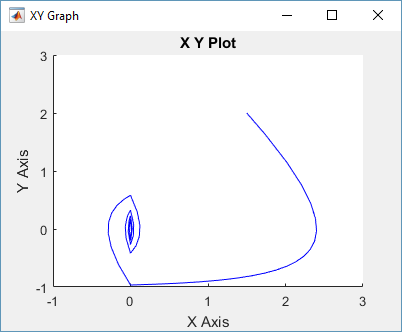
\includegraphics[height=0.4\textheight, keepaspectratio]{xynohys.png}
	\caption{Fasetraject (geen hysteresis)}
	\label{xynohys}
\end{figure}
\begin{figure}[!h]
	\centering
	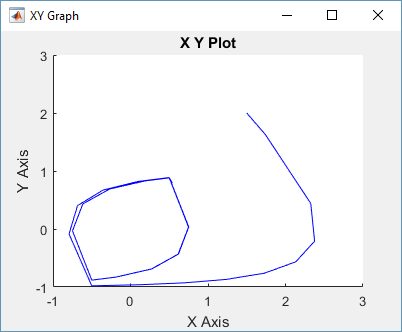
\includegraphics[height=0.4\textheight, keepaspectratio]{xyhys.png}
	\caption{Fasetraject (hysteresis)}
	\label{xyhys}
\end{figure}
\begin{figure}[!h]
	\centering
	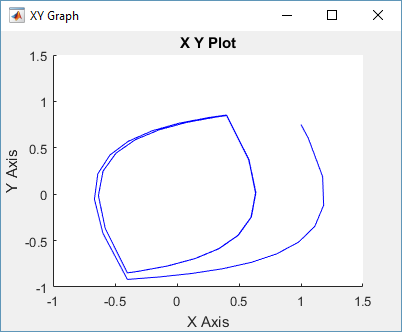
\includegraphics[height=0.4\textheight, keepaspectratio]{xytwo.png}
	\caption{Fasetraject voor $\omega_0 = 0.75$ rad/s en $\theta_0 = 1$ rad en hysteresis = $\pm 0.4$}
	\label{xytwo}
\end{figure}
\begin{figure}[]
	\centering
	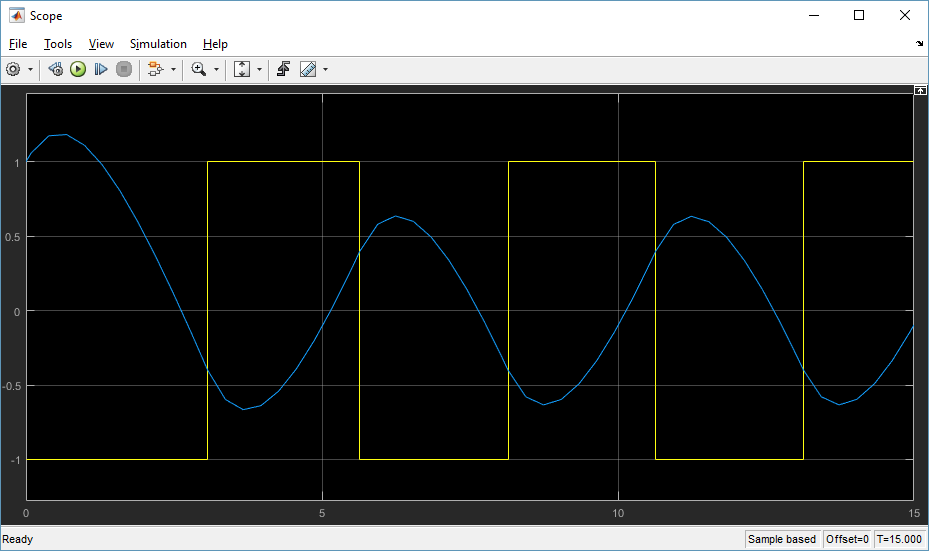
\includegraphics[width=\textwidth, keepaspectratio]{output2.png}
	\caption{Tijdrespons (15 seconden) voor $\omega_0 = 0.75$ rad/s en $\theta_0 = 1$ rad en hysteresis = $\pm 4$)}
	\label{output2}
\end{figure}



\end{document}